%\documentclass[manuscript]{aastex}
\documentclass[]{emulateapj}
%-- Packages 
\usepackage[backref, breaklinks, colorlinks, citecolor=blue, linkcolor=magenta]{hyperref}
\usepackage[dvipsnames]{xcolor}


\newcommand{\vdag}{(v)^\dagger}
\newcommand{\myemail}{n.nicole.sanchez@vanderbilt.edu}

\slugcomment{Submitted to The Astrophysical Journal}

\shorttitle{Gas Accretion in MW-like Galaxies}
\shortauthors{Sanchez et. al.}

\usepackage{natbib}
%\bibliographystyle{plain}
\bibliographystyle{apj}

\begin{document} 

\title{Preferential Accretion in the SMBH of Milky Way Size Galaxies \textcolor{green}{Due to Direct Feeding by Satellites}}
%\title{A Particular Appetite: Cosmological Hydrodynamic Simulations of Preferential Accretion in the Supermassive Black Holes of Milky Way Size Galaxies}



\author{N. Nicole Sanchez \altaffilmark{1, 2, 3}}
\author{Jillian M. Bellovary\altaffilmark{4, 5}}
\author{Kelly Holley-Bockelmann\altaffilmark{2, 3}}
\author{Michael Tremmel\altaffilmark{1}}
\author{Alyson Brooks\altaffilmark{6}}
\author{Fabio Governato\altaffilmark{1}}
\author{Tom Quinn\altaffilmark{1}}
\author{Marta Volonteri\altaffilmark{7}}
\author{James Wadsley\altaffilmark{8}}


\affil{$^1$Astronomy Department, University of Washington, Seattle, WA 98195, US, sanchenn@uw.edu}
\affil{$^2$Department of Natural Sciences and Mathematics, Fisk University, 1000 17th Avenue N., Nashville, TN 37208, USA}
\affil{$^3$Department of Physics and Astronomy, Vanderbilt University, PMB 401807, Nashville, TN 37206, USA}
\affil{$^4$Queensborough Community College, New York, NY 11364, USA}
\affil{$^5$Department of Astrophysics, American Museum of Natural History, Central Park West at 79th Street, NY 10024, USA}
\affil{$^6$Department of Physics and Astronomy, Rutgers, The State University of New Jersey, 136 Frelinghuysen Road,
Piscataway, NJ 08854, USA}
\affil{$^7$Institut d’Astrophysique de Paris, Sorbonne Universitès, UPMC Univ Paris 6 et CNRS, UMR 7095, 98 bis bd Arago, 75014 Paris, France}
\affil{$^8$Department of Physics and Astronomy, McMaster University, Hamilton, ON L8S 4M1, Canada}



% #####################################
% ############# ABSTRACT ##############
% #####################################

\begin{abstract}\label{abs:abstractlabel}

Using a new, high-resolution cosmological hydrodynamic simulation of a Milky Way-type (MW-type) galaxy, we explore how a merger-rich assembly history affects the mass budget of the central supermassive black hole (SMBH). We examine a MW-mass halo at the present epoch whose evolution is characterized by several major mergers to isolate the importance of merger history on black hole accretion. This study is an extension of Bellovary et. al. 2013, which analyzed the accretion of high mass, high redshift galaxies and their central black holes, and found that the gas content of the central black hole reflects what is accreted by the host galaxy halo. In this study, we find that a merger-rich galaxy will have a central SMBH preferentially fed by merger gas. Moreover, we find that nearly 30$\%$ of the accreted mass budget of the SMBH enters the galaxy \textcolor{green}{directly from satellites during} the two major mergers in its history, which may account for the increase of merger-gas fueling the SMBH. Through an investigation of the angular momentum of the gas entering the host and its SMBH, we determine that merger gas enters the galaxy with lower angular momentum compared to smooth accretion, partially accounting for the preferential fueling witnessed in the SMBH. In addition, the presence of mergers, particularly major mergers, also helps funnel low angular momentum gas more readily to the center of the galaxy. Our results imply that galaxy mergers play an important role in feeding the SMBH in MW-type galaxies with merger-rich histories.

\end{abstract}
\keywords{Black hole physics -- Galaxies: spiral -- Galaxies: kinematics and dynamics -- Methods: Numerical}


% ########## END OF ABSTRACT ##########
% #####################################


% #####################################
% ########## INTRODUCTION #############
% #####################################

\section{Introduction}\label{sec-intro}

Supermassive black holes (SMBHs) are thought to exist in almost all massive galaxies \citep[see][for a review]{Kormendy2013}. In the canonical picture of BH growth, these black holes may become active galactic nuclei (AGN) during periods of high accretion and wane in periods of quiescence \citep{Begelman1980,Alexander2005,Papovich2006,Volonteri2012}. The host galaxy's size, star formation rate, and other environmental effects may help to influence the growth of the black hole residing at its center; however, there are still uncertainties concerning the relationship between these SMBHs and their much larger host galaxies, as well as how they grow and evolve together \citep{Haehnelt2000,DiMatteo2005,Hopkins2006,Fu2008,Sijacki2009,Silverman2009,Micic2011,Mullaney2012}.

The M$-\sigma$ relation, which relates the SMBH's mass and the velocity dispersion of the host galaxy's central stellar population, gives some insight into the complex interplay between these objects \citep{Ferrarese2000,Gebhardt2000}. A prominent trend appears, as SMBHs tend to scale with the velocity dispersion of the host galaxy bulge. The tightness of the relation is significant and can be seen over several orders of magnitudes in velocity dispersion and black hole mass \citep[e.g.][]{Merritt2001,Tremaine2002,Graham2011,Mcconnell2013}. Scatter exists among the low mass galaxies and a deviation may appear at the high mass end, where overmassive BHs may reside \citep{VanDenBosch2007,Moster2010,Natarajan2011,Emsellem2011,Volonteri2016}. However, scatter in less massive galaxies may imply that there are several channels of black hole growth at play in the low mass end of the relation \citep{Micic2007,Volonteri2009,Reines2013,Graham2014}. One standard explanation for the M$-\sigma$ relation lies in galaxy mergers, which build up galaxies, feed SMBHs, and assemble bulges \citep[e.g.][]{DiMatteo2005,Shen2008}. Major mergers are thought to supply gas to the central SMBH resulting in feedback which quenches star formation and affects the structure of the galaxy \citep{Schawinski2010}. 

Major mergers between massive galaxies are thought to be efficient fueling mechanisms for bright AGN. \textcolor{violet}{These mergers can strongly disturb the affected galaxies producing large influxes of material due to tidal torques which can causes bursts of star formation and help funnel gas directly into the center where the SMBH resides; however, while major mergers remain a viable process for large scale inflows of gas into the host galaxy, there is still some uncertainty regarding the processes that transport gas through last $\sim$ 1 kpc to the SMBH} \citep[e.g.][]{Sanders1988,Sanders1996,Barnes1991,Mihos1996,Hopkins2006,Richards2006,Reddy2008,Hopkins2010}. Additionally, the most massive, highest-luminosity AGN (i.e. quasars) reside in incredibly luminous infrared galaxies where star formation is abundant, signifying that major mergers may have recently occurred \citep{Treister2012}. Distorted morphologies are often characteristics of quasar hosts, and companions can also be present around quasars, both of which are evidence that strengthen the possibility of a recent merger having affected their lifetimes \citep{Ellison2010}. 

In many less massive and less luminous AGN, however, there is a clear lack of distorted morphology, close neighbors, and/or other obvious merger evidence \citep{Ryan2007,Schawinski2011,Ellison2013,Hicks2013}. It is also important to note that many of these AGN exist in spiral galaxies, which are unlikely to have been recently disturbed by major mergers \citep{Schawinski2011,Kocevski2011}. Nevertheless, some evidence suggests that disturbed galaxies may reform a disk quickly, even after a major merger, as long as it is gas-rich \citep{vanGorkom1997}. The rapid disk reformation of the galaxy in this paper was previously studied by \cite{Governato2009} (See \ref{results}). More recently, \cite{Treister2012} has suggested that only the highest luminosity AGN require fueling via major mergers; $\sim$ 90 $\%$ of AGN across all redshifts are fueled by various other mechanisms, which may include minor mergers, flybys, and smooth accretion, whereby gas is directly accreted via large filaments from the ambient intergalactic medium \citep{Cox2006,Bellovary2013,Sinha2012,Dubois2012,DiMatteo2016}.

Smooth accretion, in particular, may play an important role in fueling these low mass galaxies. Halos less than 10$^{11}$ $M_{\odot}$ can accrete filaments of unshocked gas; thereafter, gas will shock heat to the virial temperature of the halo \citep{Keres2005}. Even for massive halos, unshocked gas may still penetrate shocked regions to fuel the galaxy \citep{Brooks2009,Dekel2009,Nelson2013}. In addition, SMBH feedback, the depositing of energy and angular momentum back into the gas reservoir during accretion, also affects the overarching structure of the host galaxy \citep{Governato2009a}. Secular processes, including bar formation and disk instabilities, may also be prominent forms of accretion for these SMBHs \citep{Athanassoula2016,Kormendy2013}. 

It is clear that galaxy hosts grow through a variety of channels that depend on mass, environment, and interaction history. Therefore, we want to understand how these different galaxy evolutionary paths translate into SMBH fueling mechanisms, and see how they affect the fueling gas flowing into the SMBH itself. \cite{Bellovary2013} compared simulations of three high mass, high redshift galaxies and found that while mergers and smooth accretion both efficiently build up galaxies, no particular dynamical process was more adept at feeding the SMBH. However, with only minor mergers, these galaxies represented relatively quiet merger histories. Using a similar method as \cite{Bellovary2013}, this work examines the SMBH and galaxy fueling mechanisms of a MW-mass galaxy with a rich merger history. MW-type galaxies host SMBHs on the order of 10$^6$ $M_{\odot}$, which are likely the most common type of massive black hole, yet little is known about them or how they may grow \citep{Kormendy2013}. Through this examination, we hope to better understand the coevolution of SMBHs and their hosts in this class of galaxy. 

In this study we analyze the Milky Way-type galaxy, h258, which has a history characterized by major mergers. Since this galaxy is similar to the MW in virial mass, stellar mass, and circular velocity, without a deeper examination, we may not recognize the turbulent history from which it results. We will pinpoint the origins of gas entering the SMBH and halo to look for clues about SMBH fueling within this galaxy. By examining its assembly, and its SMBH's fueling, we can determine the accretion rate and gain further understanding about how SMBHs grow over a range of merger histories in galaxies like our own.

% ####### END OF INTRODUCTION #########
% #####################################


% #####################################
% ####### SIMULATION PARAMETERS #######
% #####################################

\section{Simulation Parameters}\label{sec-model}

Using the smoothed particle hydrodynamics (SPH) N-body tree code, Charm N-body GrAvity solver \citep[ChaNGa;][]{Menon2015}, we ran an initial dark matter-only, uniform resolution volume of 50 h$^{-1}$ Mpc on a side to identify a MW-mass halo at z = 0 for further examination. This DM-only simulation assumed WMAP 3 parameters \citep{Spergel2007}: $\Omega_m$ = 0.24, $\Omega_{\Lambda}$ = 0.76, $H_0$ = 73 km/s, and $\sigma _8$ = 0.77. Halo h258 was chosen for its Milky Way-mass at z=0 and its active merger history. The halo has a virial mass of $M_{\rm vir} = 7 \times 10^{11} M_{\odot}$ at z = 0 defined relative to a critical density, $\rho_c$, where $\rho / \rho_c$ = 100. Two recent major mergers characterize the h258 halo at z=1.8 and z=1.2. We constructed a ``zoom-in'' high resolution simulation on this galaxy, including gas and star particles, using the volume-renormalization of \cite{Katz1993}, resimulating only a few virial radii from the main halo at the highest resolution from z=150 to z=0.  

We note that a lower resolution version of h258 was run using the Gasoline code \citep{Wadsley2004}. Our higher resolution h258 run has a spline force softening length of 174 pc and initial gas particle masses of 2.7 $\times$ $10^4 M_{\odot}$. Star particles are created with 30$\%$ of their parent gas particle mass, allowing a maximum initial mass of 8100 $M_{\odot}$. Halo h258 contains about 5 million DM particles inside the virial radius at z=0 and over 14 million DM, star, and gas particles total. The resolution of both force and mass in these simulations is comparable to the ``Eris'' simulation which has one of the highest resolutions for an N-body+SPH cosmological simulation of a Milky Way-mass galaxy so far produced \citep{Guedes2011}.  

Compared to the previous h258 simulation, the ChaNGa simulated h258 scales better and includes a new improved SPH formalism \citep{Keller2014}. The hydrodynamic treatment now includes a geometric density average\textemdash (P$_i$ + P$_j$)/($\rho_i \rho_j$) rather than P$_i$/$\rho_{i}^2$ + P$_j$/$\rho_{j}^2$ where P$_i$ and $\rho_i$ are the particle's pressure and density\textemdash in the force expression, in addition to the standard SPH density estimator \citep{Ritchie2001}. Adjusting the force expression diminishes the numerical surface tensions due to shear flows, such as Kelvin-Helmholtz instabilities. We also apply a consistent and entropy-conserving energy equation to account for the modified force expression and correctly model strong shocks, such as Sedov blasts.

Our simulation introduces a uniform UV background at z$\sim$9 to simulate the cosmic reionization energy energy using the formula of \cite{Haardt2012}. To model star formation, we stochastically turn gas particles into stars with a star formation efficiency parameter of c$^*$ = 0.1 once the density threshold and temperature satisfy conditions for star formation (10.0 amu cm$^{-3}$; T \textless 10$^4$ K).  \textcolor{green}{As shown in \citet{Governato10}, this high density threshold is necessary to produce bursty star formation events in the high-density peaks of the ISM.  Realistic star formation histories result in galaxies which have realistic density profiles and lie on the observed scaling relations (mentioned in detail below).  The lower-resolution simulations mentioned in this paper have a lower threshold, since the high density peaks are not resolved.}
These star particles represent a Kroupa initial mass function \citep{Kroupa1993}.  Molecular hydrogen and metal-line cooling are not included, though we implement a low-temperature extension to the cooling curve to trace metals \citep{Bromm2001} and the metal diffusion prescription of \cite{Shen2010}. 
 

Supernova (SN) feedback releases $10^{51}$ ergs of thermal energy within a ``blastwave'' radius determined by the equations of \cite{Ostriker1988}. In the affected region, cooling turns off for a time relative to the expansion phase of the SN remnant also determined by the blastwave equation. SN Ia and II rates from \cite{Thielemann1986} and \cite{Woosley1995}, respectively, are implemented through the \cite{Raiteri1996} method, which uses the stellar lifetime calculations of the Padova group \citep{Alongi1993, Bressan1993, Bertelli1994} to describe stars with varying metallicities. Both the supernova ``blastwave'' radius and supernova (Ia and II) prescriptions are described in detail by \cite{Stinson2006}. \textcolor{violet}{While \textcolor{green}{it is true that} a different treatment of the \textcolor{green}{ISM and }SNe feedback might alter the structure of the ISM, \cite{Christensen2014} examined simulated spiral and dwarf galaxies utilizing similar SNe prescriptions \textcolor{green}{and three different ISM models,} and determined that the resulting ISM remained consistent with each other. Additionally, our galaxy is in good agreement with galaxies affected by superbubble SN feedback \citep{Keller2014}.}

Simulated galaxies are shown to conform with the observed Tully-Fisher relation \citep{Governato2009}, the size-luminosity relation \citep{Brooks2011}, and the mass-metallicity relation \citep{Brooks2007,Christensen2015}, in addition to having realistic matter distributions and baryon fractions \citep{Governato2009a,Guedes2011}. The parameter and resolution choices described above allow the galaxies to adhere to the stellar-mass-halo-mass relation at z=0 and maintain a realistic period of star formation \citep{Moster2010,Munshi2013,Brooks2007,Maiolino2008}. Given that the simulations are in accordance with observations, we are confident that it reasonably represents growth in the galaxy and its SMBH.
 
Since there are uncertainties in black hole seed formation, we model BH seeding that is broadly consistent with several theories of direct collapse black holes \citep{Couchman1986, Abel2002, Bromm2004} and Population III stellar remnants \citep{Loeb1994, Eisenstein1995, Koushiappas2004, Begelman2006, Lodato2006}. While this method allows the BH formation process to remain physically motivated, BH seeds form if their parent gas particle matches the criteria required for star formation and also maintains zero metallicity, a requirement of many direct collapse models. A probability of $\chi_{\rm seed}$ $\sim$ 0.1 is applied to determine whether a gas particle (with the above specifications) will become a BH seed with the same mass as its parent gas particle. This probability was chosen to match the predicted occupation fraction of BH seeds at z $\sim$ 3 \citep{Volonteri2008}.

The requirement that BH seeds must form from zero metallicity gas particles also causes BH formation to be confined in areas of primordial star formation in the earliest and most massive halos in the simulation. In this technique, BH formation is dependent only on local environment, neglecting any large-scale properties of the host halo. We use the sub-grid prescription for modeling the effects of dynamical friction on SMBH orbits from \cite{Tremmel2015}, which has been shown to produce realistic sinking times for SMBHs.  This prescription, combined with our high resolution to minimize two-body interactions and numerical noise, results in SMBHs that can remain stable at galactic center while also, when appropriate, experiencing realistic perturbations and sinking timescales during and after galaxy interactions and mergers \citep{Bellovary2011}.

Black hole mergers occur when they are separated by less than twice the softening length and satisfy $(1/2) \delta v^2 < \delta a \cdot \delta r$ (which is an approximation of being gravitationally bound),  where $\delta v$ and $\delta a$ are the velocity and acceleration differences between the two black holes and $\delta r$ is the distance separating them. In addition to gaining mass via mergers, black holes accrete through the Bondi-Hoyle mechanism:
\begin{equation}
\dot{M} = \frac{4 \pi \alpha G^2 M^{2}_{\rm BH} \rho}{(c^{2}_{s} + v^2)^{3/2}},
\end{equation}
where $\alpha$ is a constant of order 1, $\rho$ is the density of the surrounding gas, $c_s$ is the sound speed, $v$ is the black hole's relative velocity to the gas, and the accretion rate is Eddington-limited. Feedback is applied to surrounding gas with an energy boost determined by the accreted mass as follows: $\dot{E}$ = $\epsilon _{r}$$\epsilon_{f}$$\dot{M}$$c^2$ where $\dot{M}$ is the accreted mass, and $\epsilon _r = 0.1$ and $\epsilon _f = 0.03$ are assumed for the radiative efficiency and feedback efficiency, respectively. This energy is distributed as thermal energy to the 32 nearest particles via a kernel probability function. Though other groups use a higher value for feedback, $\epsilon _f = 0.05$ \citep{Sijacki2007,DiMatteo2008}, we find that $\epsilon_f = 0.03$ in our code produces massive black holes (MBHs) in better agreement with MBH-host galaxy scaling relations. However, as our main concern is in the relative proportion of gas from various origins (See \ref{results}) and we restrict our analysis of the angular momentum of gas to only the timestep of entry into the main halo, our results are not sensitive to our choices of $\epsilon _{r}$ or $\epsilon_{f}$. This same model was additionally used by \cite{Bellovary2013} at a lower resolution and without the addition of the dynamical friction prescription. 

% ### END OF SIMULATION PARAMETERS ####
% #####################################


% #####################################
% ######### REDUCTION METHOD ##########	
% #####################################

\section{Simulation Analysis}\label{redux}

We first identify halos using the Amiga Halo Finder which uses an overdensity criterion for a flat universe \citep{Knebe2001,Knollmann2009,Gill2004} to set the virial radius in the primary halo. We select the primary halo to be the most massive at z=0 in the high resolution region. The central SMBH in the primary halo has a mass of $1.3 \times 10^{7} M_{\odot}$ \textcolor{violet}{and a velocity dispersion in the bulge of $\sigma$ $\sim$ 152 km s$^{-1}$, indicating that h258 lies on the M-$\sigma$ relation.}

In this analysis, we retrace each gas particle that was accreted by the galaxy or SMBH, following the gas back through its journey in the galaxy and recording its host halo and time of accretion \citep{Brooks2009}. The particles are then classified into types by their method of entrance into the primary halo. In particular, gas particles are classified as ``early'' if they exist in the primary halo before z $\sim$ 16. Gas that belonged to a different halo than the primary prior to accretion is classified as ``clumpy,'' entering the primary halo through mergers. All other gas is classified as ``smooth'' accretion, and is then subdivided into two categories: ``unshocked'' and ``shocked.'' Unshocked gas will usually flow into the halo via large-scale, dark matter filaments \citep{Keres2005,Bellovary2013}. It is possible for unshocked gas to be dense enough to pierce an already developed shock, allowing it to funnel into the galaxy core where it can be accreted onto the SMBH \citep{Nelson2013}. 

However, as we discussed in Section 1, if the galaxy halo is $\gtrsim$ 10$^{11}$ M$_{\odot} $, the gas is known to shock-heat to the virial temperature of the halo. We identify shocked particles through an increase in entropy and temperature using the following criteria:
\begin{equation}
T_{\rm shock} \geq 3/8 T_{\rm vir},
\end{equation}
where T$_{\rm vir}$ is the virial temperature of the halo, T$_{\rm shock}$ is the temperature of the gas particle, and 
\begin{equation}
\Delta S \geq S_{\rm shock} - S_0,
\end{equation}
where S$_0$ is the initial entropy of the gas particle, and 
\begin{equation}
S_{\rm shock} = log_{10}[3/8 T_{\rm vir}^{1.5}/4 \rho_0],
\end{equation}
where $\rho_0$ is the gas density prior to the shock. Since our halo is $\sim$ 10$^{12}$ M$_{\odot} $ by z = 0, we should expect to find more shocked gas entering the halo at later times. Both types of smoothly accreted gas are tracked until they reach a cutoff radius at 10$\%$ of the virial radius (0.1 R$_{vir}$) at which point supernova feedback may appear as virial shocking and cause contamination in our estimates of shocked accretion. This cutoff also accounts for any AGN feedback we might encounter.

Once all the gas particles have been individually categorized, we can use these labels to classify the gas accreted by the SMBH, and we can better contrast the processes that feed the galaxy and its SMBH in MW-mass halos.

% ###### END OF REDUCTION METHOD ######
% #####################################


\begin{figure}
\centerline{\resizebox{0.75\hsize}{!}{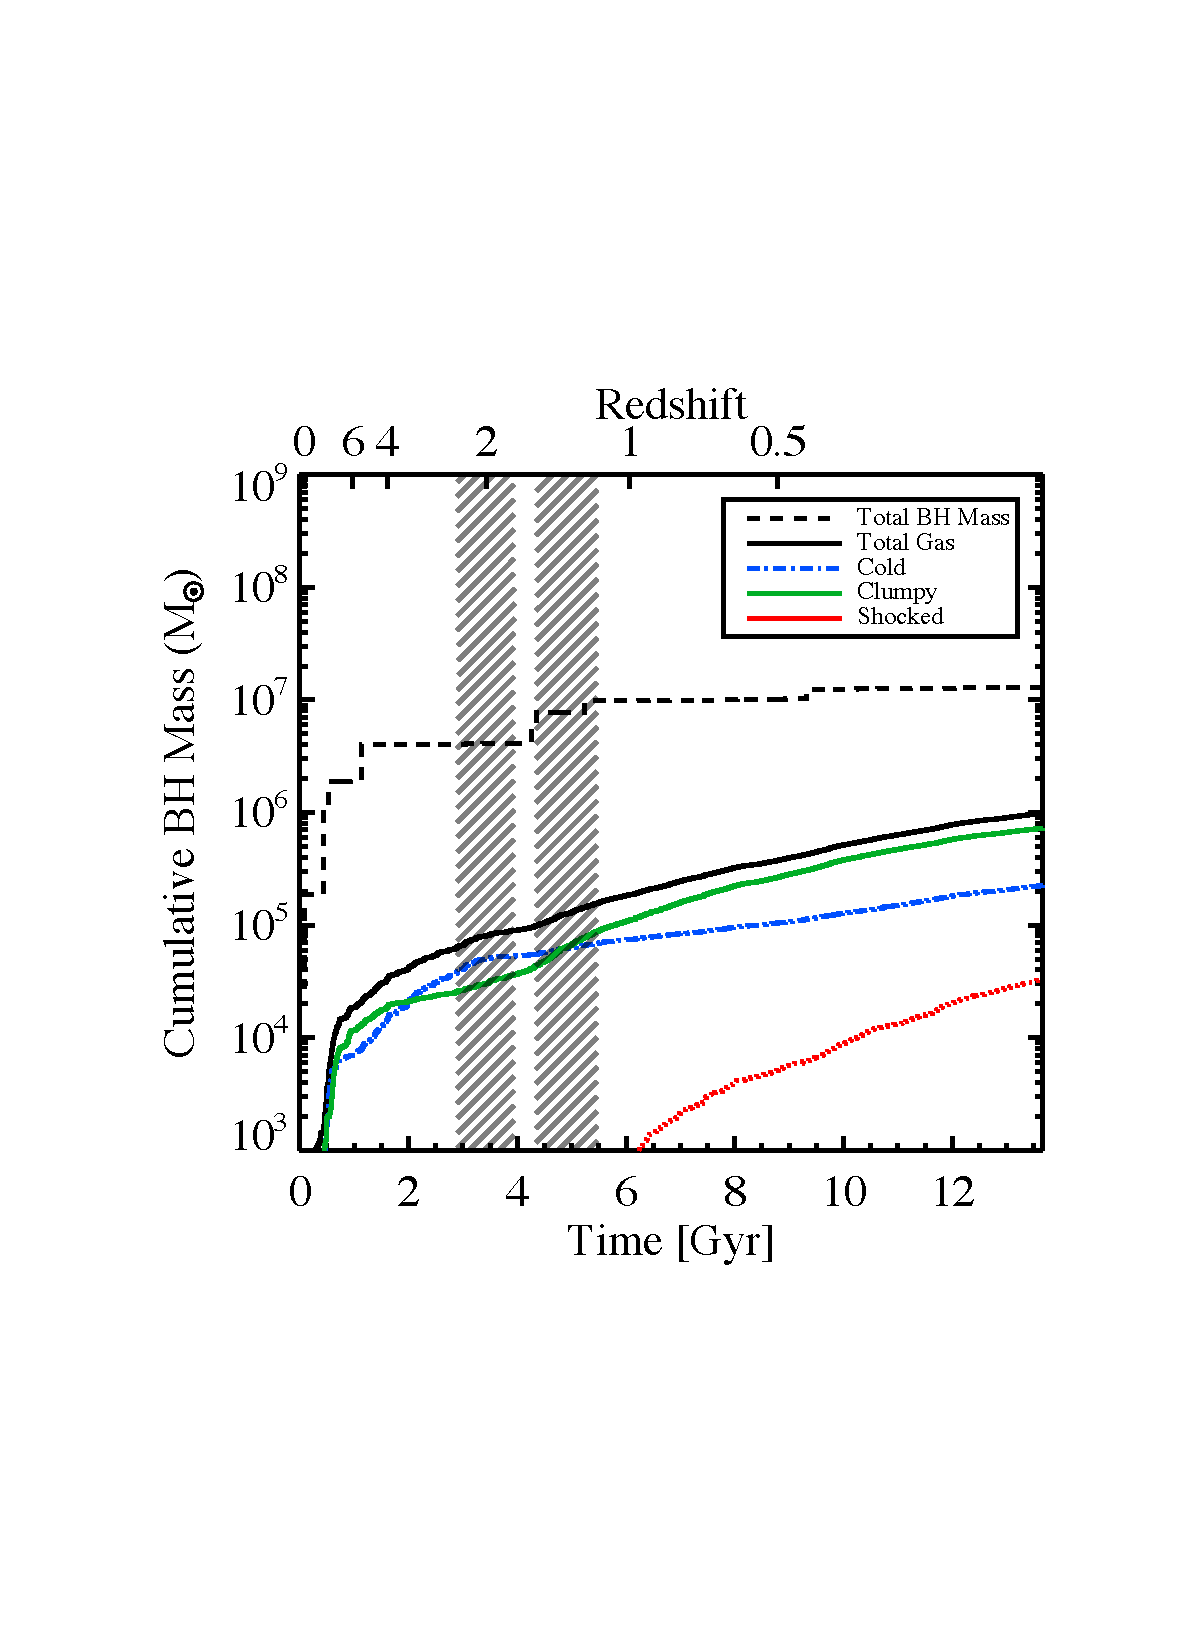
\includegraphics[angle=0]{hrh258_massgastime_hashed.pdf}}}
\caption[]{The central BH's cumulative mass as a function of time and redshift. The black dashed line indicates the total cumulative BH mass. The black solid line indicates the total accreted gas mass. The blue dot-dashed line indicates smoothly accreted gas mass that remains unshocked after entering the virial radius of the main halo. The green solid line indicates the gas mass accreted through mergers. The red dashed line indicates accreted gas mass that was shocked upon entry into the halo. \textcolor{violet}{Major mergers are marked with grey hatched regions.}}
\label{hrh258allmassgas} 
\end{figure}

\begin{figure}
\centerline{\resizebox{0.75\hsize}{!}{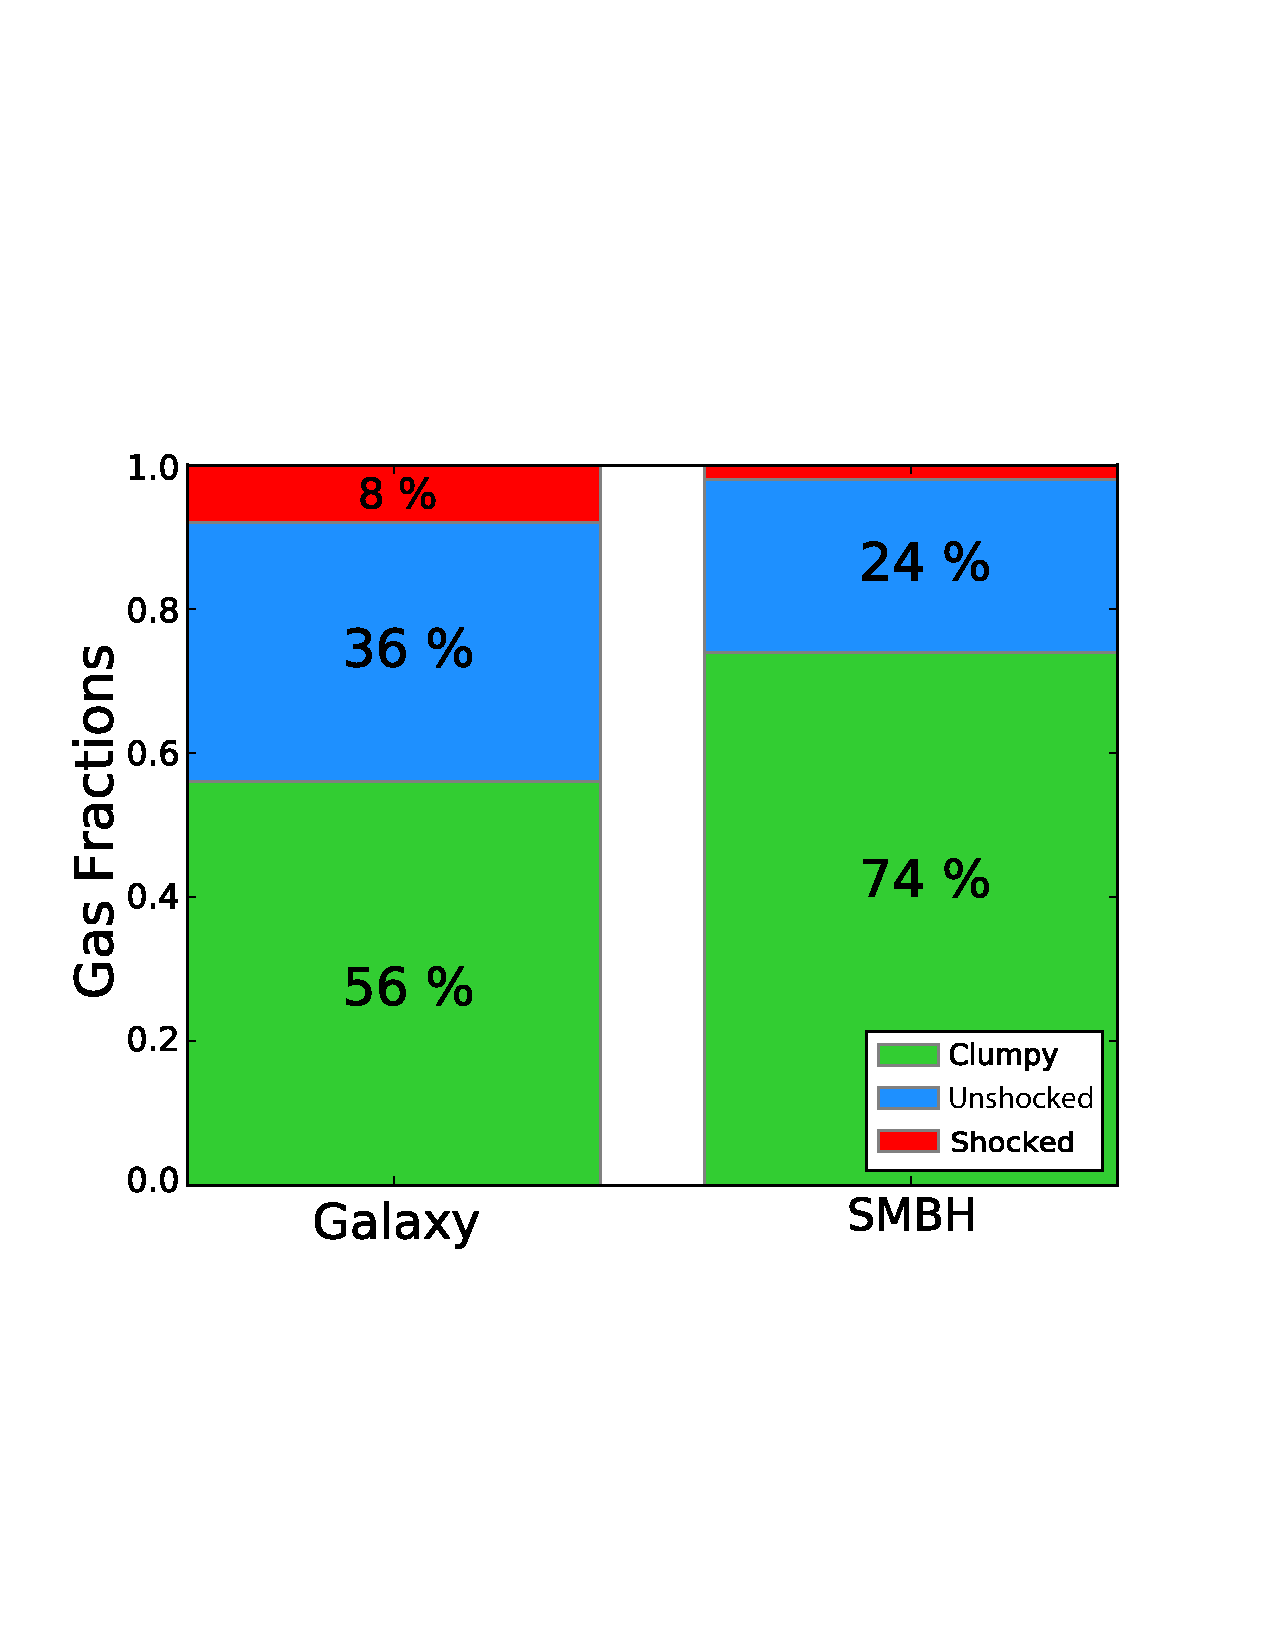
\includegraphics[angle=0]{hrh258_stackbarfractions.pdf}}}
\caption[]{Gas fractions of the gas particles accreted by the main halo (left) and the SMBH (right), distinguished by type. Blue, green, and red distinguish gas gained via smooth accretion that remains unshocked, gas gained through mergers, and smoothly accreted gas that is shocked upon entry, respectively.}
\label{hrh258stackfrac}
\end{figure}


% #####################################
% ############# RESULTS ###############
% #####################################

\section{Results} \label{results}

% ########## HI RES H258 ############
%\subsection{ChaNGa - High Resolution h258}

The galaxy h258 is characterized by two major mergers; the first occurs at z $\sim$ 1.8 (mass ratio, q $\sim$ 0.8) and the second at z $\sim$ 1.2 (q $\sim$ 1). Despite its merger-rich history, gas accretion smoothly increases the cumulative black hole mass in h258 throughout its evolution as can be seen in Figure \ref{hrh258allmassgas}. The black dashed line in \ref{hrh258allmassgas} indicates the total cumulative BH mass (including both mass from gas and BH mergers), while the black solid line indicates the total accreted gas mass. The blue dot-dashed line represents the gas mass accreted via unshocked gas, while the green solid line and red dashed line show the gas mass accreted through mergers and shocked gas, respectively. \textcolor{violet}{Major mergers are indicated by grey hatched regions.} It is worthwhile to point out that the largest part of the mass budget at high redshift is not gas at all, but other black holes that have merged with the SMBH seed. This has important implications for gravitational wave astronomy, increasing the event rate for SMBH assembly at high redshifts \citep{Holley-Bockelmann2010}. Aside from this early BH assembly, the largest gain in accreted SMBH mass comes from gas associated with the major mergers between z $\sim$ 2 and z $\sim$ 1. We know unshocked gas makes up the majority of accreted mass entering the galaxy at early times; however, the transition between when smooth, unshocked accretion and merger gas dominates are clearly distinguished. While clumpy gas (green) dominates gas mass accretion in the SMBH at the earliest time, unshocked gas (blue) overtakes it for a short time before clumpy gas once again dominates by z $\sim$ 1.5. 

This low redshift transition to a clumpy gas preference results in the large fraction of clumpy gas seen in the accreted mass fractions in the SMBH (Figure \ref{hrh258stackfrac}). Figure \ref{hrh258stackfrac} depicts the fractions of total gas accretion in the galaxy and the SMBH at z=0, again differentiated by gas origin. The gas accreted by the galaxy is half (56 $\%$) comprised of merger gas, with 36 $\%$ of the gas entering through unshocked, smooth accretion. The smallest fraction of the total gas is comprised of shocked gas (8 $\%$ ). Unlike the galaxy, nearly three quarters (74 $\%$) of the gas accreted by the central SMBH was accreted via mergers, while only a quarter (24 $\%$ ) is comprised of unshocked, smoothly accreted gas. Shocked gas makes up the last 2$\%$ of total gas entering the SMBH. \textit{It is evident then that the SMBH more readily accretes gas gained through mergers. While this result is consistent with the work of \cite{Dubois2015} which explores how galaxy mergers may be necessary for triggering black hole growth in low mass galaxies, it} is contrary to \cite{Bellovary2013} which found that in high redshift, high mass galaxies, the fractions of gas comprising the SMBH and its host were nearly the same. Through our results, it appears that when major mergers are a key part of the galaxy assembly history, these mergers may also drive SMBH growth.

To examine why mergers feed the SMBH so effectively, we focus on the most major mergers (q \textgreater 0.8), which occur at  z$\sim$1.8 and z$\sim$1.2 and involve the third and second largest halos in the zoom-in simulation, respectively. We also examine the major mergers' solitary effects on the SMBH mass budget. By tracing the gas particles that enter the main halo from these two specific halos, we can determine what mass fraction of those particles would eventually accrete onto the SMBH. We chose a timestep for each merging halo prior to the start of its individual merger and selected the gas particles associated with them. We selected the gas particles associated with the second largest halo at z$\sim$1.5 and the gas particles associated with the third largest halo at z$\sim$2.5. Tracing the gas particles from these two timesteps into their mergers with the main halo, we found that 28$\%$ of total mass budget of the SMBH was comprised of the gas from these major mergers. Considering that 74 $\%$ of the SMBH's accreted gas mass is composed of clumpy gas, this implies that more than a third of the total clumpy gas in the SMBH comes from these two major mergers. From the previous study \citep{Bellovary2013}, we might have thought the SMBH's mass budget would have been comprised of ~56$\%$ clumpy gas since the halo's accreted mass budget is 56$\%$; however, the 28$\%$ of accreted gas entering the SMBH from the secondary and tertiary halos can explain the increase in the overall clumpy fraction of the SMBH's mass budget.

A previous study by \cite{Fu2007} supplies direct observational evidence that gas from a merger can be funneled directly into the vicinity of the SMBH (\textless 1 pc). Their study examined a collection of twelve low-redshift quasars, half of which are characterized by luminous extended emission-line regions (EELRs). These EELRs were found to have metallicities below the mass-metallicity correlation of normal galaxies and are thought to have resulted from massive, galactic superwinds accompanying the creation of the powerful radio jets associated with the quasars. The quasars hosting EELRs were also found to have low-metallicity broad-line regions (BLRs) at their centers, while the quasars without EELRs hosted BLRs with metallicities above Z$_{\odot}$. \cite{Fu2007} determined that the presence of these low-metallicity EELRs as well as the similar, low-metallicity BLRs are evidence of a merger with a gas-rich galaxy. Such an interaction may explain both the infusion of low-metallicity gas into the BLRs and the subsequent ejection of that gas by the radio jets, forming the EELRs.  While our study did not measure metallicity or include radio jets, our overall results support the conclusion that a majority of the gas from the secondary and tertiary galaxy mergers directly fuel the SMBH at the center of the primary galaxy. 

\begin{figure}
\centerline{\resizebox{0.75\hsize}{!}{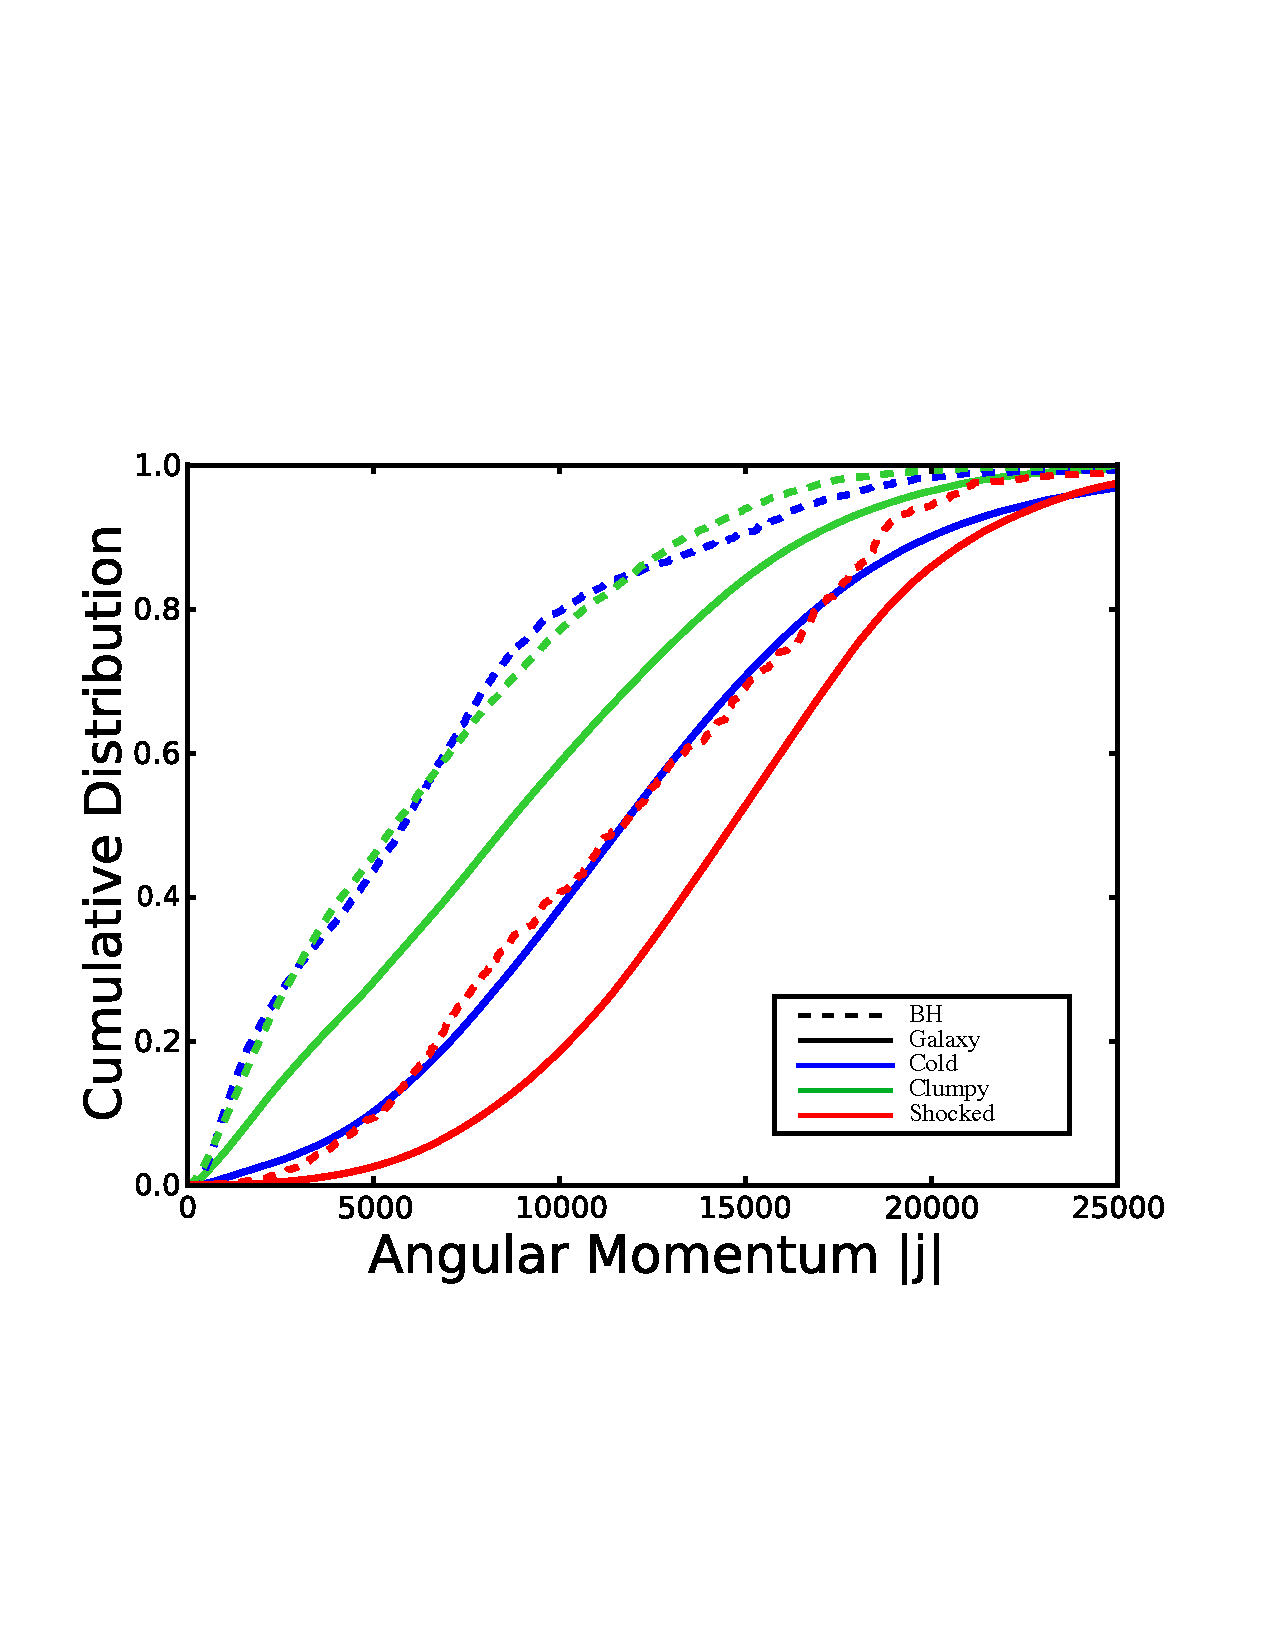
\includegraphics[angle=0]{hrh258_am_cumu_4096_legend.pdf}}}
\caption[]{ Normalized cumulative distribution of angular momentum (kpc km s${{-1}}$) of the gas particles accreted onto h258 by z = 0.  Gas particles accreted onto the main halo (solid lines) and central black hole (dashed lines). The green, blue, and red lines indicate clumpy, unshocked, and shocked gas, respectively.}
\label{hrh258angmom} 
\end{figure}

\begin{figure}
\centerline{\resizebox{0.75\hsize}{!}{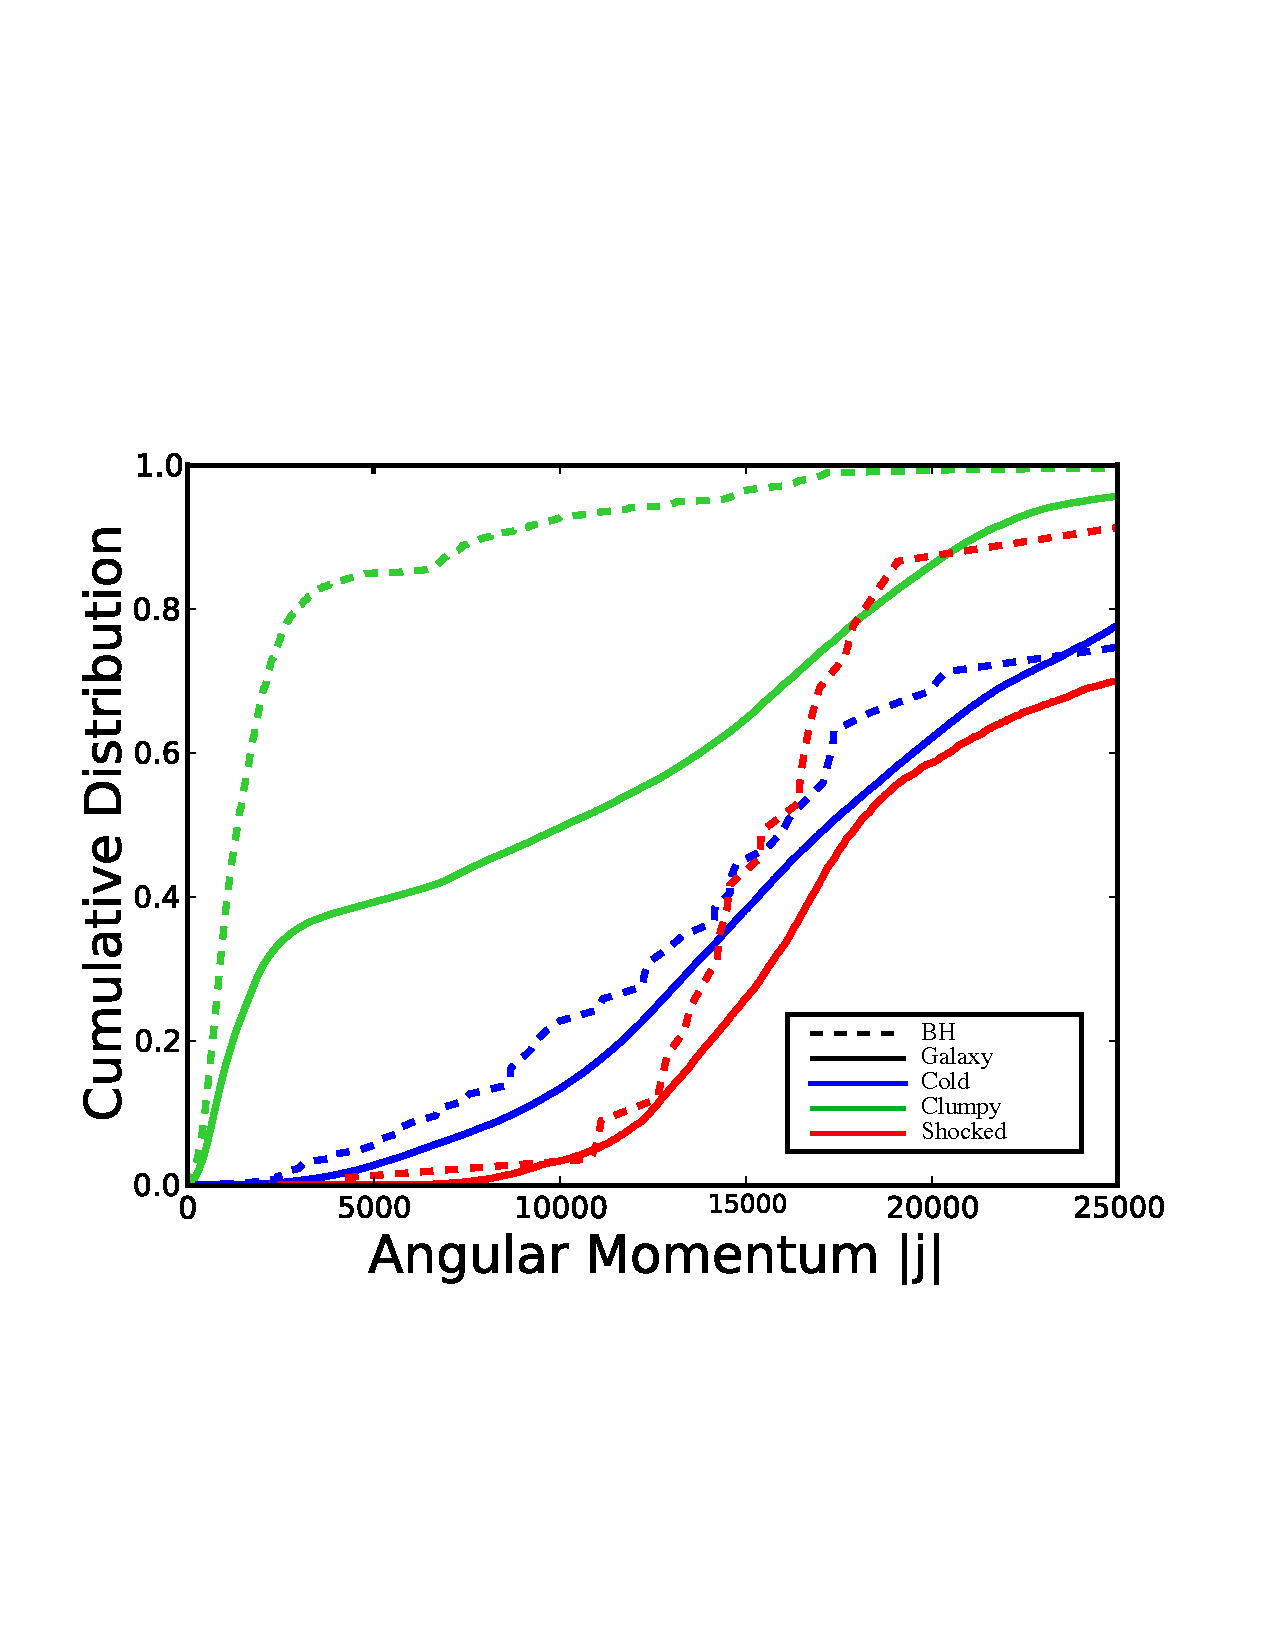
\includegraphics[angle=0]{hrh258_am_tsnew_1584_legend.pdf}}}
\caption[]{ Normalized cumulative distribution of angular momentum (kpc km s${{-1}}$) of the gas particles accreted onto the h258 galaxy at a single timestep (z $\sim$ 1.2) during the major merger's greatest influx of accreted gas. About 450,000 gas particles accreted onto the halo at this timestep. Angular momentum of gas particles accreted onto the main halo and central black hole are distinguished by solid and dashed lines, respectively. The green, blue, and red lines indicate clumpy, unshocked, and shocked gas, respectively.}
\label{hrh258angmom_merger2} 
\end{figure}

To better understand the apparent preference for merger-accreted gas, we examine the angular momentum of the gas at the moment it enters the halo. Figure \ref{hrh258angmom} shows a cumulative distribution of the angular momentum of the gas as it enters the halo (solid lines). We further distinguish the gas that enters the SMBH (dashed lines), still considering its angular momentum at the moment of halo entry. The gas is again distinguished by origin (clumpy, unshocked, shocked being green, blue, and red, respectively). We find that the angular momentum of gas entering which eventually reaches the SMBH is lower overall, and that the lowest angular momentum gas is comprised of both clumpy and unshocked gas. This result can be seen in Figure \ref{hrh258angmom_merger2}, which shows the cumulative distribution of the angular momentum of the incoming gas particles at the time of the greatest influx of accreted gas during the merger at z $\sim$ 1.2. (Colors and linestyles as in Figure \ref{hrh258angmom}.) Figure \ref{hrh258angmom_merger2} explicitly shows that the gas ending up in the SMBH enters with the lowest angular momentum. This influx of clumpy gas primarily had its origins in the secondary halo. Examining the angular momentum of all the gas entering from the secondary halo, we found that it was consistent with the angular momentum of the total clumpy gas entering the main halo.  Thus it appears that gas from the secondary galaxy may be directly channeled into the SMBH of the primary, in addition to the standard picture of gas in the host galaxy which loses angular momentum due to torques from the merger dynamics \citep{Capelo2015}, 

A lower resolution version of the galaxy h258 was run using the N-body code, Gasoline, like the simulations in \cite{Bellovary2013}. Despite fundamental differences in the hydrodynamic implementation and gas physics included and the absence of a dynamical friction prescription, an analysis of this low resolution h258 results in a SMBH with the same distinct preference for accreting clumpy gas. A second galaxy, h277, was also run using Gasoline; however, this galaxy was characterized by a quiescent merger history (no major mergers) and resulted in a SMBH whose accreted mass fractions mirrored the halo (as seen in \cite{Bellovary2013}). The broad consistency between the low and high resolution simulation of the same galaxy, and the similar results of a quiescent galaxy to the previous study, indicates that the large scale gravitational dynamics could be a main driver of the SMBH fueling in this case. We also stress that that while major mergers may not be the only physical mechanisms by which gas can be funneled into the centers of galaxies (the previous study being a strong example of this), mergers between galaxies clearly play an important role when considering the gas accretion of SMBHs.


% ########## END OF RESULTS ###########
% #####################################


% #####################################
% ########### CONCLUSION ##############
% #####################################

\section{Conclusion}
%\textcolor{violet}{
This study examines the gas accretion onto the fully cosmological simulation of a Milky Way-size galaxy to redshift z $=$ 0, with major mergers characterizing its past. We trace the gas into the SMBH at its center and differentiate the gas accreted onto the galaxy and SMBH by origin. Gas gained through mergers is classified as ``clumpy'' gas and smoothly accreted gas is separated into ``shocked'' and ``unshocked'' categories. Our goal is to determine what types of gas are primarily feeding the SMBH and the galaxies of this class, and to determine what effects the merger history of a galaxy may have on these processes.
%}

%\textcolor{violet}{
A previous study by \cite{Bellovary2013} analyzed high mass, high redshift galaxies and found the gas composition of the SMBHs mirror their host. Contrary to these previous results, when we examined a galaxy with an active merger history, we determined that the SMBH at the center more readily accretes gas gained through mergers. This remained true both in an older low resolution simulation of the same galaxy as well as this current iteration. \textit{In both the low and high resolution cases, we see a significant increase in the clumpy gas accreted by the SMBH compared to its host.} We also note that in the high resolution case, we can attribute the increase of clumpy gas to the major mergers that characterize h258. 
%}

The angular momentum of the accreted gas as it enters the galaxy sheds some light on the mechanism driving this preferentially accreted clumpy gas. Smoothly accreted gas, which enters the galaxy with a wide range of angular momentum, is likely to adjust to the net angular momentum of the halo gas; however, some studies have found that low angular momentum gas can fuel the central SMBH via filaments of smoothly accreted gas \citep{Dubois2012,DiMatteo2016}. Meanwhile, gas entering through mergers can fall to the galaxy's center with minimal interaction with the halo gas. This restriction gives gas accreted through mergers the advantage of falling more readily to the center and accreting onto the SMBH. Considering all origins of gas, our study is the first to see a clear contribution to gas from merging galaxies directly feeding the SMBH.
%%%% INSERT DYNAMICAL FRICTION DISCUSSION HERE JILLIAN %%%%%

While the examination of this single, extreme case of a galaxy with an active merger history depicts a class of galaxy with varying SMBH accretion methods, a further study of cases with varying merger histories is required to begin understanding the broad spectrum of Milky Way-mass galaxy accretion \citep{Pontzen2016}. Additionally, examinations of other extreme case, e.g. galaxies with varied but still merger-rich histories, may strengthen the validity of this result. Through this study, we show that the presence of major mergers can play an important role in the final compositions of central SMBHs, but the question of how important these mergers are remains to be seen.
%}

% ####### END OF CONCLUSIONS ##########
% #####################################


\acknowledgments
%\textcolor{violet}{
Resources supporting this work were provided by the NASA High-End Computing (HEC) Program through the NASA Advanced Supercomputing (NAS) Division at Ames Research Center. Results were partially obtained using the analysis software Pynbody (https://github.com/pynbody/pynbody). We thank the Fisk-Vanderbilt Masters-to-PhD Bridge program for the funding and support of this research. JB acknowledges generous support from the Helen Gurley Brown Trust. M.V. acknowledges support from NASA award ATP NNX10AC84G.

\bibliography{/Users/the_neekster/Documents/MENDELEY/MEND_bibtexfiles/Sanchez2016.bib}

\end{document}

